\documentclass{article}
\usepackage[T2A]{fontenc}
\usepackage[utf8]{inputenc}
\usepackage[russian]{babel}
\usepackage{amsmath,amssymb,amsthm,enumitem,fourier, empheq}
\usepackage{exercise}
\usepackage{pgf,tikz}
\usepackage{pgfplots}
\usepackage{graphicx}
\usepackage{circuitikz}

\usetikzlibrary{arrows}
\usetikzlibrary{circuits}

\title{Теория вероятностей}
\author{Ле Куок Зунг}
\date{\today}

\theoremstyle{definition}
\newtheorem*{exercise}{Упражение}

\begin{document}
	\maketitle
	\section*{Занятия 2}
\begin{exercise}[1] Десять команд случайным образом (по жребию) разбиваются на две разные подгруппы. 
	
	$| \Omega | = C^5_{10} C^5_5$
	
	\begin{enumerate}
		\item [(a)] Выбрать место для 2 сильнейших команд: 2 \\ Выбрать 4 команда для подгруппы 1: $C^4_8$ \\ Выбрать 4 команда для подгруппы 2: $C^4_4$ \\ Ответ: $\frac{2 C^4_8 C^4_4}{C^5_{10} C^5_5} = \frac{5}{9}$
		\item [(б)] Выбрать подгруппу для 2 команда: $C^1_2$ \\ Выбрать больше 3 команда этой группы: $C^3_8$ \\ Ответ: $\frac{C^1_2 C^3_8}{C^5_{10} C^5_5} = \frac{4}{9}$
		\item [(в)] Выбрать больше 3 команда первой группы: $C^3_8$ \\ Выбрать 5 команд второй группы: $C^5_5$ \\ Ответ: $\frac{C^3_8 C^5_5}{C^5_{10} C^5_5} = \frac{2}{9}$
	\end{enumerate}
\end{exercise}

\begin{exercise}[2]
	\begin{enumerate}
		\item [(а)] $| \Omega | = C^3_{52}$ \\ Выбрать тройку $C^1_4$, семарку $C^1_4$, туз $C^1_4$ \\ Ответ: $\frac{C^1_4 C^1_4 C^1_4}{C^3_{52}} = \frac{16}{5525}$
		\item [(б)] $| \Omega | = A^3_{52}$ (так как мы выберем последовательные карты) \\ Для три любых карт существует только один заказ, поэтому нужно выбрать атрибут первой карты $C^1_4$, второй $C^1_4$, третьей $C^1_4$ \\ Ответ: $\frac{C^1_4 C^1_4 C^1_4}{A^3_{52}} = \frac{8}{16575}$
	\end{enumerate}
\end{exercise}

\begin{exercise}[3]
	\begin{tikzpicture}
		\draw (-4,0) -- (4,0);
		\filldraw [black] (-4,0) circle (2pt) node[anchor=south]{$O$};
		\filldraw [black] (-2,0) circle (2pt) node[anchor=south]{$B$};
		\filldraw [black] (1.5,0) circle (2pt) node[anchor=south]{$C$};
		\filldraw [black] (4,0) circle (2pt) node[anchor=south]{$A$};
	\end{tikzpicture}
	
	Пусть $L$ - длина отрезка $OA$ \\ $x$ - длина отрезка $OB$ \\ $y$ - длина отрезка $BC$ \\ У нас есть: $\begin{cases}
		y < x \\ x +y < L \\ x > 0 \\ y > 0
	\end{cases}$
	
	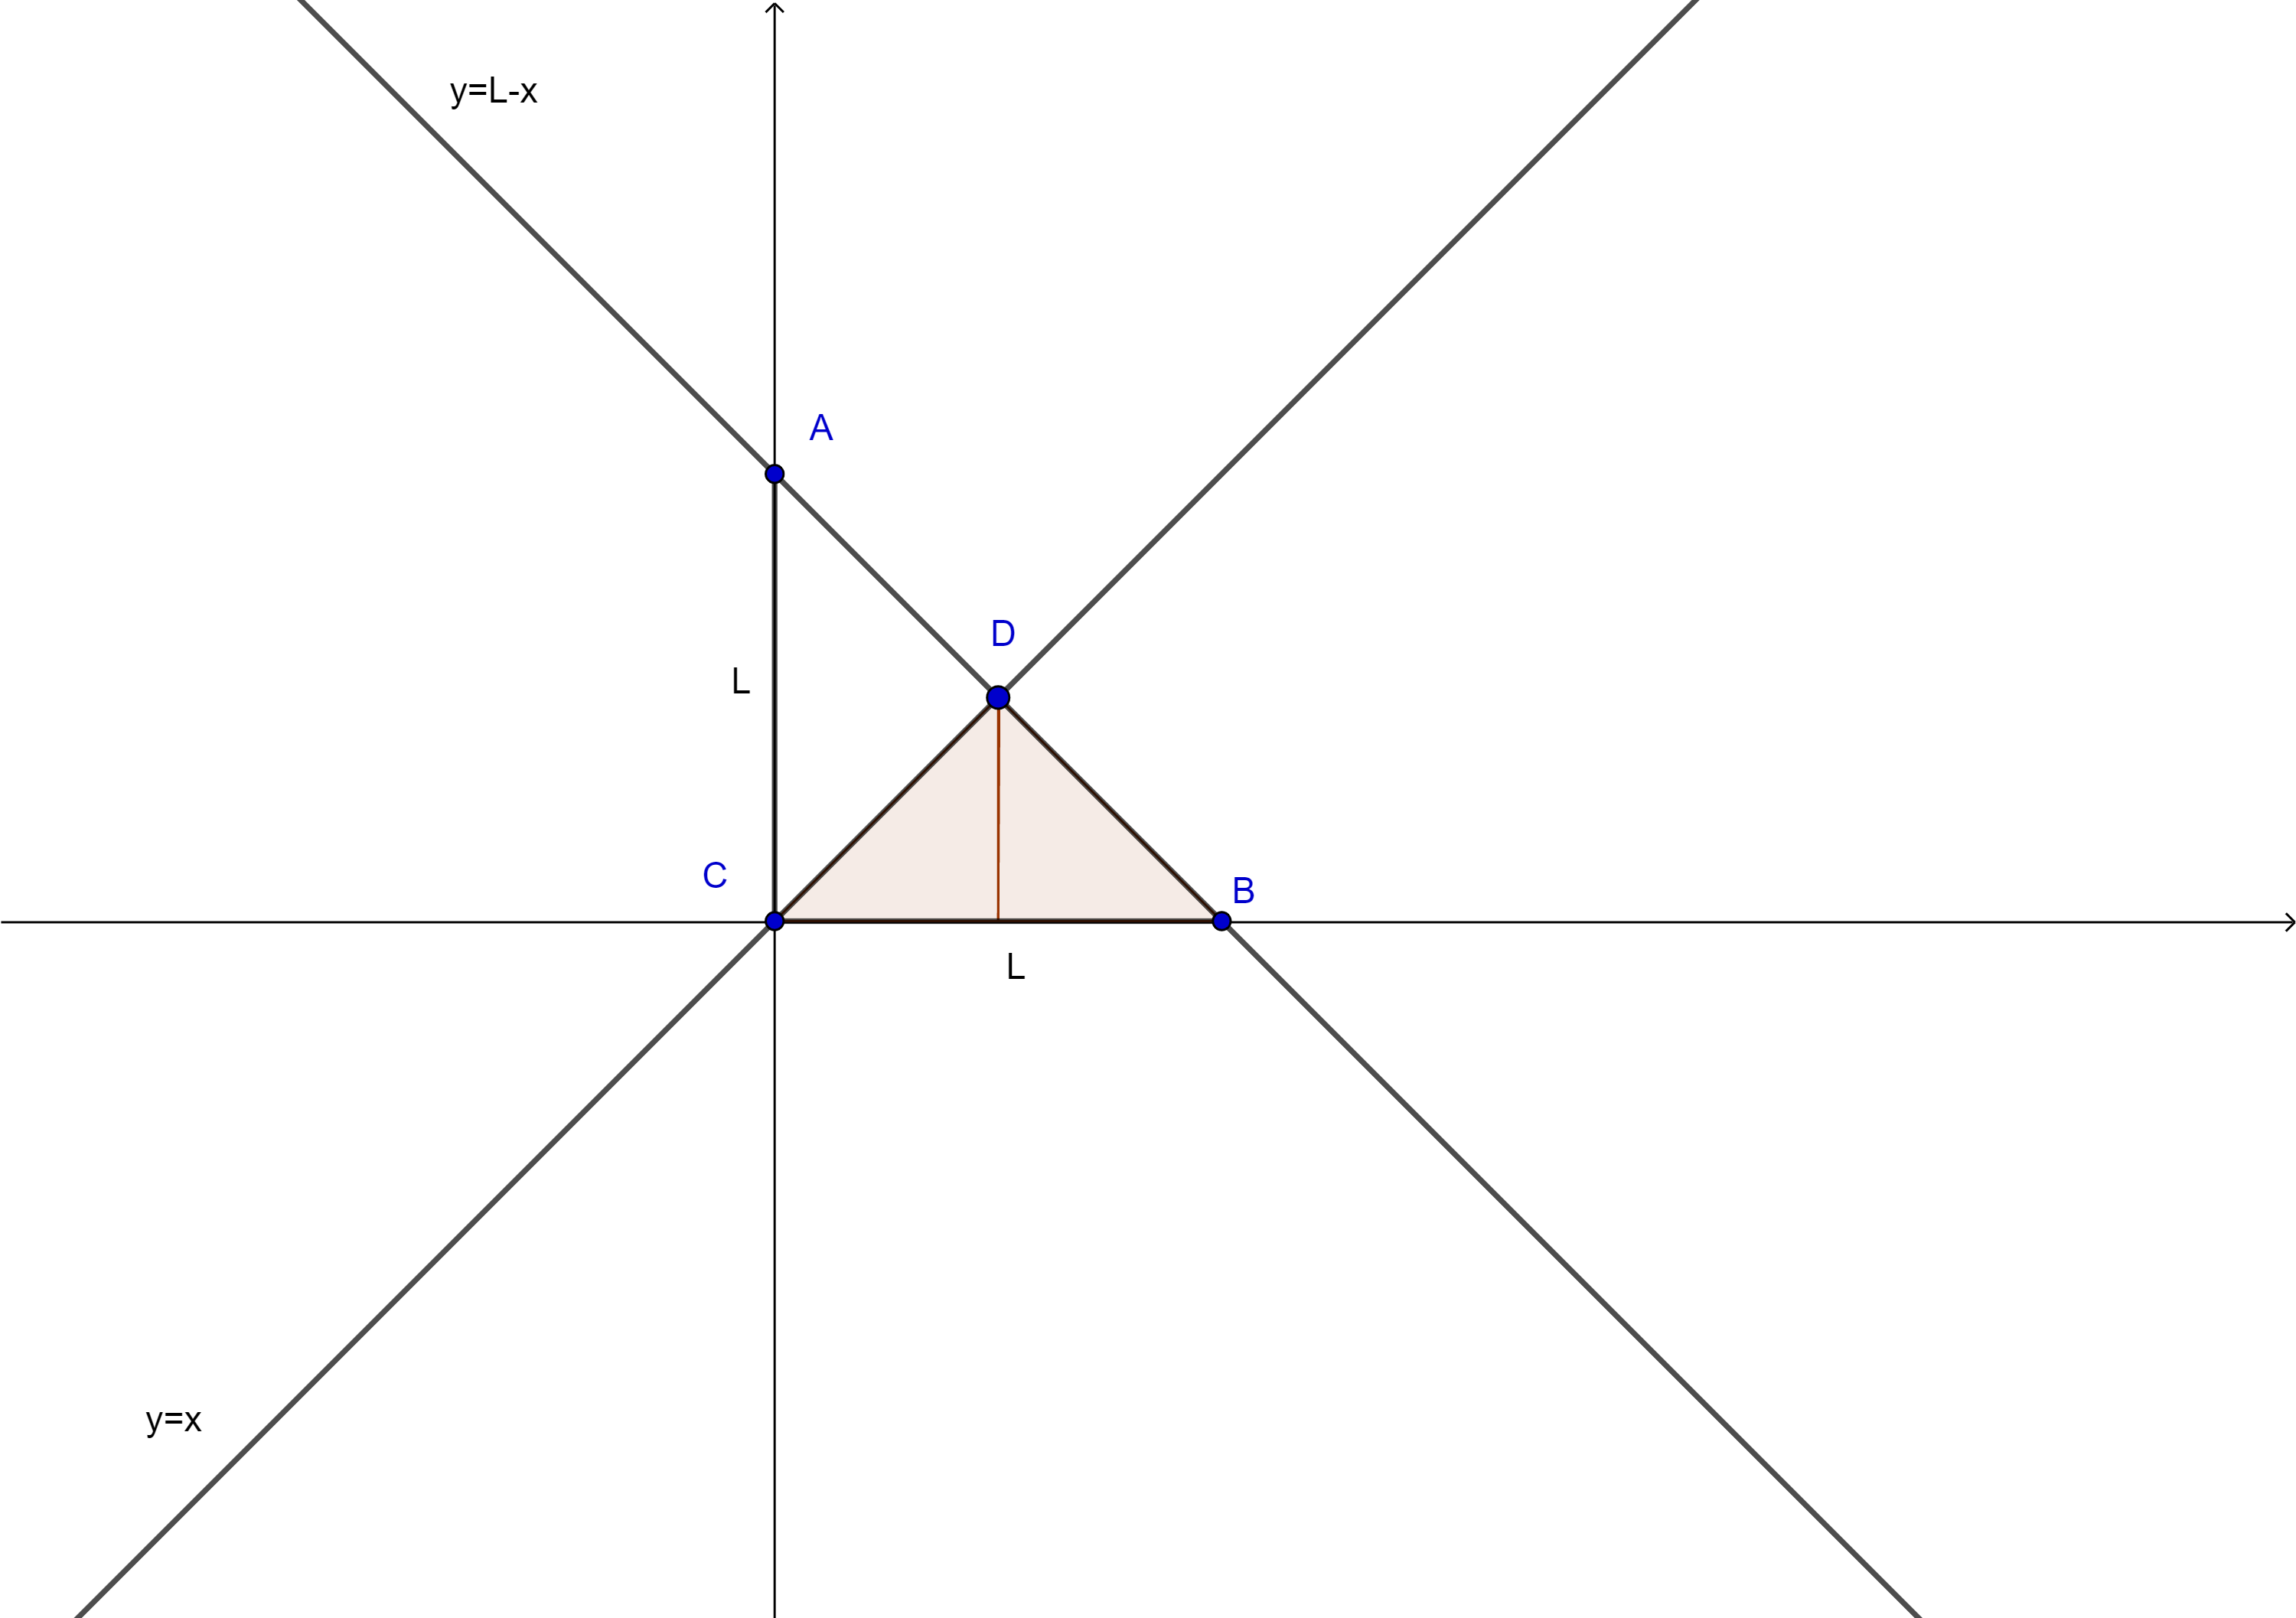
\includegraphics[width=\textwidth]{exercise3-2.png}	
	
	Здесь, $| \Omega | = \frac{L^2}{2}$, а вероятность, которая удовлетворяет условии: $\frac{L \cdot \frac{L}{2}}{2} = \frac{L^2}{4}$ \\ Ответ: $\frac{L^2}{4} : \frac{L^2}{2} = \frac{1}{2}$
\end{exercise}

\begin{exercise}[4]
	$| \Omega | = 10!$ \\ Ответ: $\frac{1}{10!}$
\end{exercise}

\begin{exercise}[5]
	$| \Omega | = 8^4$
	\begin{enumerate}
		\item [(a)] Выбрать 4 этажа из 8: $A^4_8$ \\ Ответ: $\frac{A^4_8}{8^4} = \frac{105}{256}$
		\item [(б)] Этаж 6, 7, 8, 9, поэтому 4 этажа: $4^4$ \\ Ответ: $\frac{4^4}{8^4} = \frac{1}{16}$
		\item [(в)] 7 этажов: $7^4$ \\ Ответ: $\frac{7^4}{8^4} = \frac{2401}{4096}$
	\end{enumerate}
\end{exercise}

\begin{exercise}[6]
	$| \Omega | = 10^4=10000$
	\begin{enumerate}
		\item [(a)] Первое число имеет 9 вариантов (кроме 0). Другие числа имеют 10 вариантов \\ Ответ: $\frac{9 \cdot 10^3}{10^4} = 0,9$
		\item [(б)] Чтобы делится на 5, последнее число равно 0 или 5 \\ Ответ: $\frac{9 \cdot 10^2 \cdot 2}{10^4} = 0,18$
	\end{enumerate}
\end{exercise}

\begin{exercise}[7]
	$| \Omega | = C^{10}_{20}$ \\ Если билеты 1 и 2 не будет, тогда имеется 18 билетов, значит $C^{10}_{18}$ \\ Ответ: $\frac{C^{10}_{18}}{C^{10}_{20}} = \frac{9}{38}$
\end{exercise}

\begin{exercise}[8]
	$| \Omega | = C^4_{6+4+2} = C^4_{12}$ \\ Ответ: $\frac{C^4_{4+2}}{C^4_{12}} = \frac{1}{33}$
\end{exercise}

\begin{exercise}[9]
	$| \Omega | = 10!$ \\ 
	Рассмотрим 3 красного книги как 1, тогда у нас нес 8 книг. Найти места для 8 книг: $8!$ \\ 3 краного книга имеет $3!$ \\ Ответ: $\frac{8! 3!}{10!} = \frac{1}{15}$
\end{exercise}

\begin{exercise}[10]
	Каждая кость имеет 6 вариантов, поэтому $| \Omega | = 6^3$ \\ События А: кости выпадут разными гранями, то есть $6 \cdot 5 \cdot 4$ \\ Тогда, $P(A) = \frac{6 \cdot 5 \cdot 4}{6^3} = \frac{5}{9}$ \\ События B: на всех костях выпадет одинаковое число очков, то есть 6 чисел \\ Тогда $P(B) = \frac{6}{6^3} = \frac{1}{36}$
\end{exercise}

\begin{exercise}[11]
	У нас есть 5 пар ботинок, значит 10 ботинок. Поэтому $| \Omega | = C^2_{10}$ \\ Существуют 5 пар, то $P(A) = \frac{5}{C^2_{10}} = \frac{1}{9}$
\end{exercise}

\begin{exercise}[12]
	Тат как каждый участник может получит любый приз, поэтому $| \Omega | = 10^6$ \\ Данные 6 учасников получат по одному призу каждый, то $6!$ \\ Ответ: $\frac{6!}{10^6} = 0,00072$
\end{exercise}

\begin{exercise}[13]
	$| \Omega | = C^4_8 C^4_4$ \\ Выбрать 2 юношей и 2 девушек для группы 1: $C^2_4 C^2_4$ \\ Ответ: $\frac{C^2_4 C^2_4}{C^4_8 C^4_4} = \frac{18}{35}$
\end{exercise}

\begin{exercise}[14]
	\item [(a)] $P(A) = \frac{S_{\square}}{S_{\circ}} = \Big(\frac{2R}{\sqrt{2}}\Big)^2:(\pi R^2) = \frac{2}{\pi}$
	\item [(б)] $P(B) = \frac{S_{\triangle}}{S_{\circ}} = \Big[(R \sqrt{3})^2 \cdot \frac{\sqrt{3}}{4}\Big] : (\pi R^2) = \frac{3 \sqrt{3}}{4 \pi}$
\end{exercise}

\begin{exercise}[15] В течение суток к причалу независимо друг от друга
	
	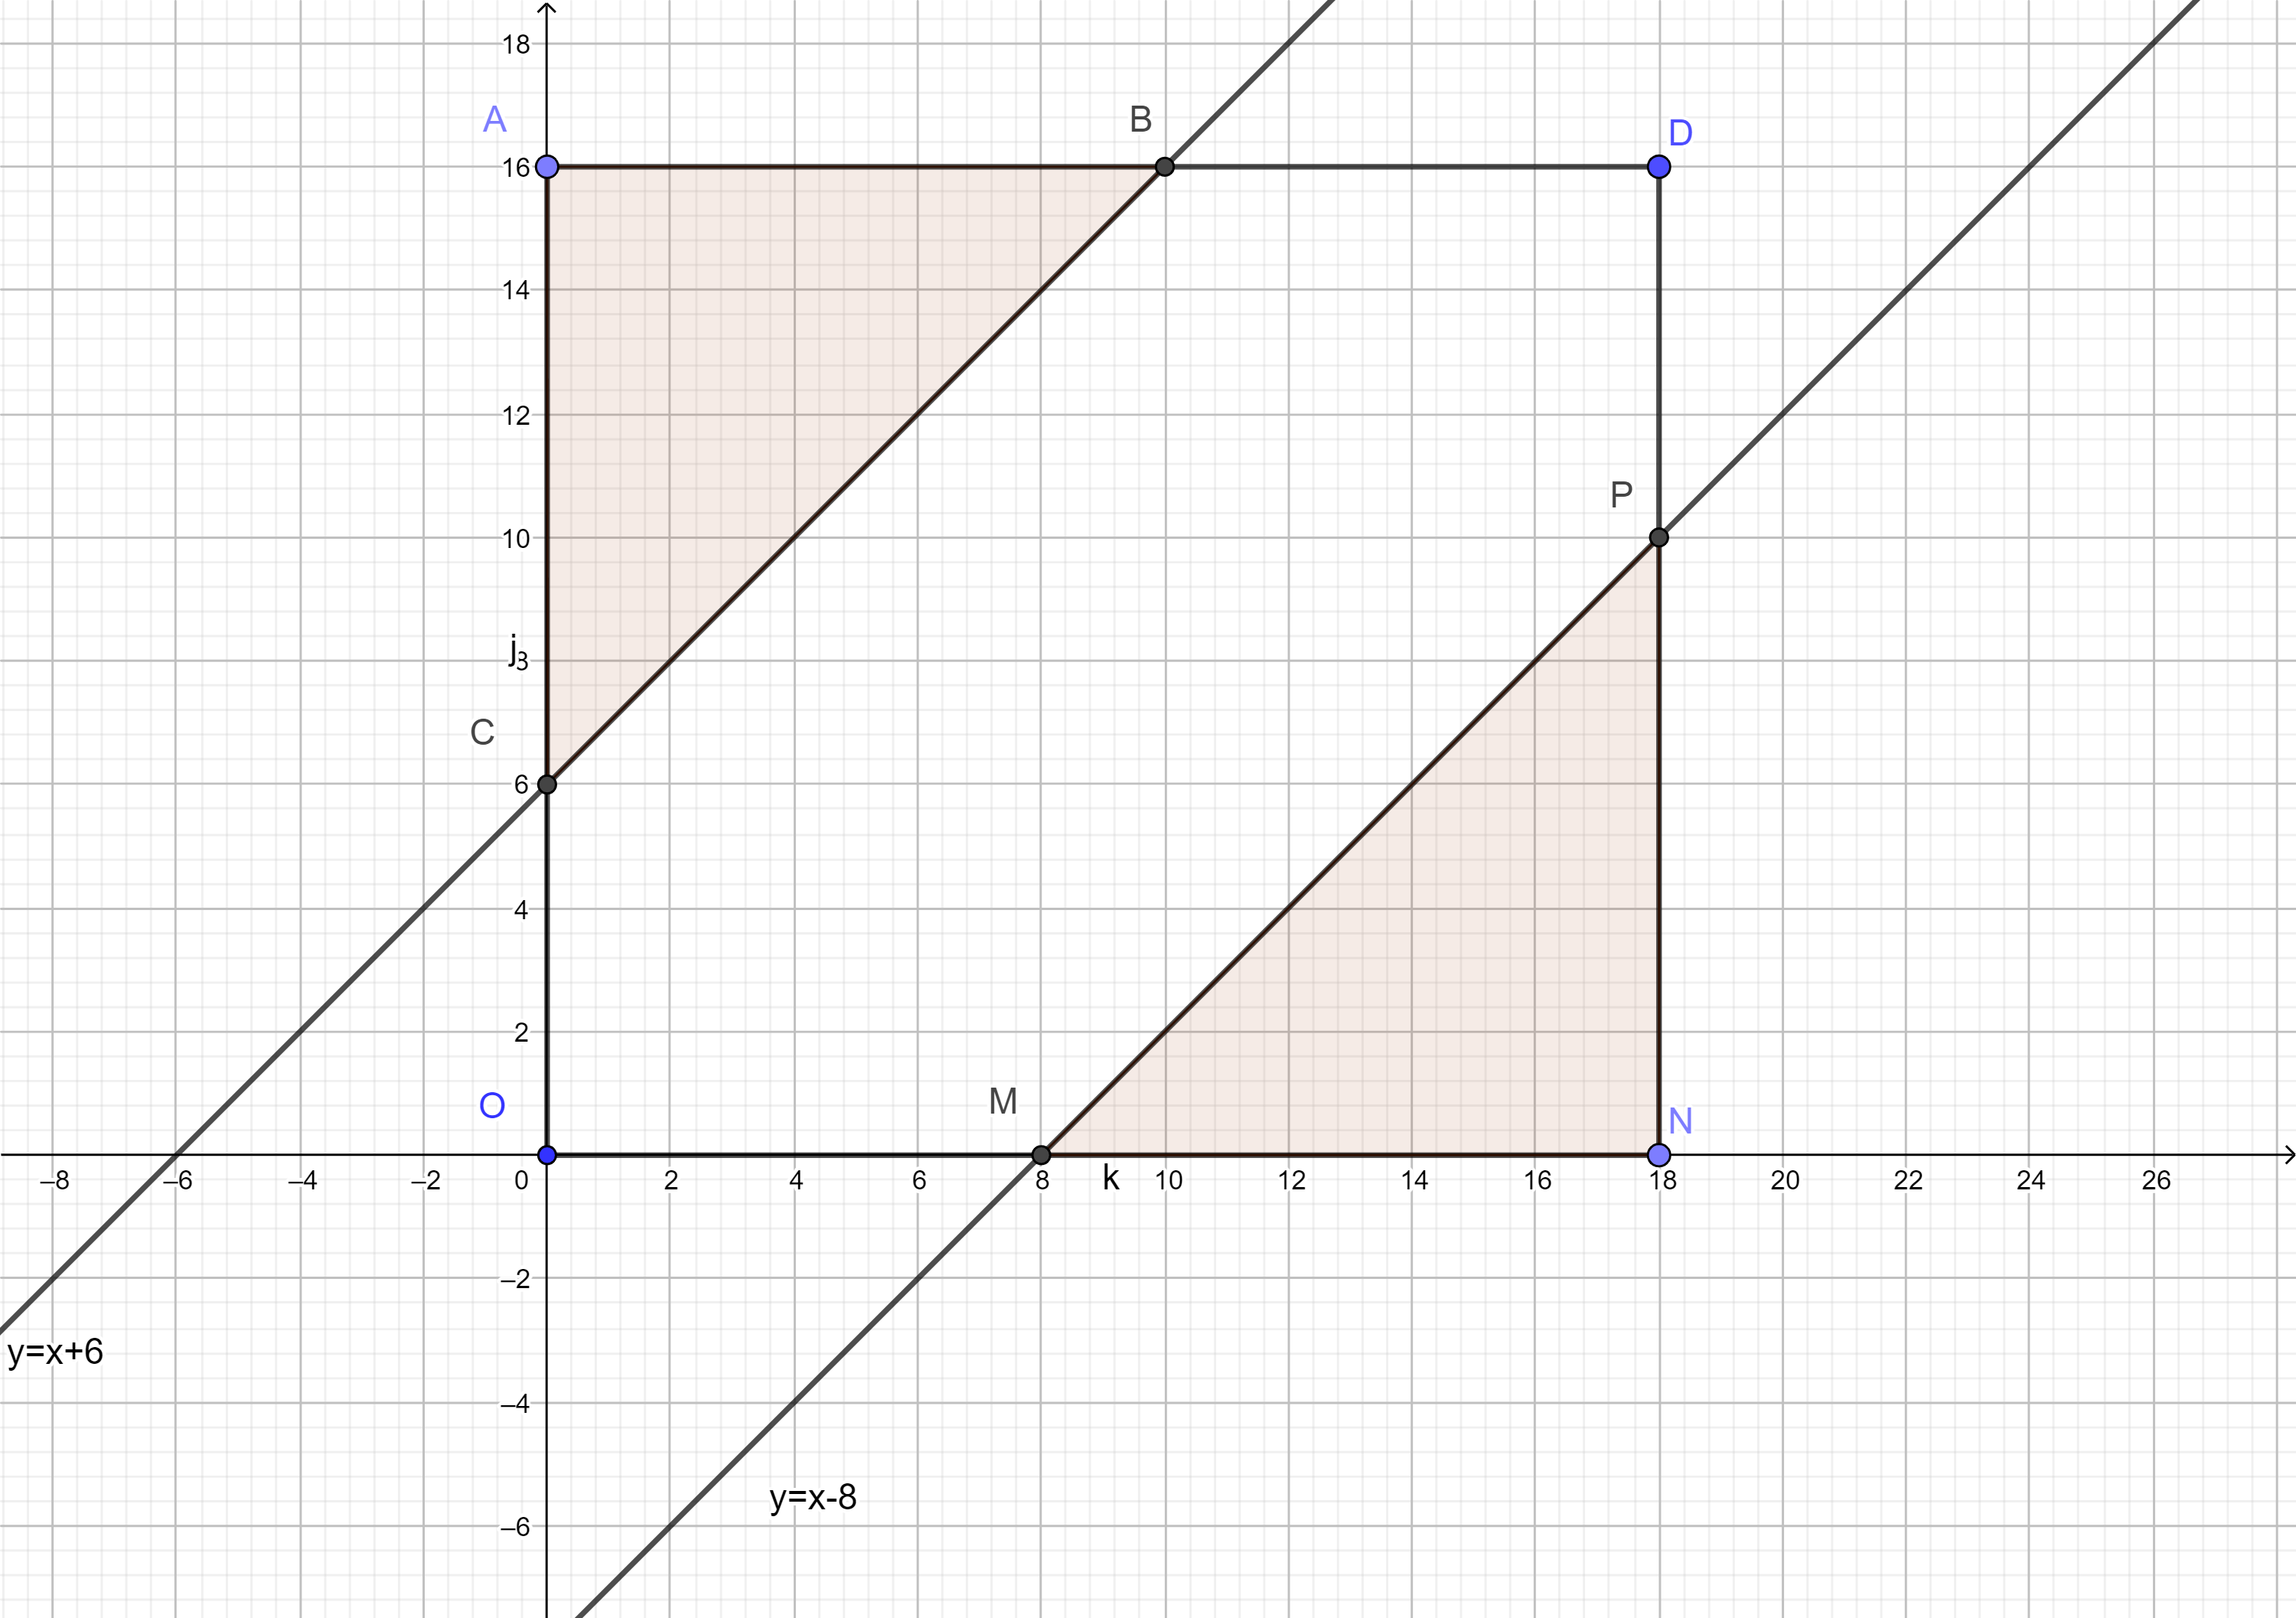
\includegraphics[width=\textwidth]{exercise15-2.png}
	
	Пусть $x$ - время первый сухогруз начинает разгрузиться и $y$ - время второй сухогруз начинает разгрузиться \\ Тогда, $x+6 \leq 24$ и $y+8 \leq 24 \Leftrightarrow x \leq 18$ и $y \leq 16$ \\ Cлучай 1: первый сухогруз начинает раньше чем второй, тогда $x+6 \leq y$ \\ Случай 2: второй сухогруз начинает раньше чем первый, тогда $y+8 \leq x$ \\ Получим $P(A) = \frac{S_{\triangle ABC} + S_{\triangle MNP}}{S_{ADNO}} = \Big(\frac{10 \cdot 10}{2} + \frac{10 \cdot 10}{2} \Big) : (16 \cdot 18) = \frac{25}{72}$ 
\end{exercise}
	\section*{Занятие 3}
\begin{exercise}[1]
	
	\begin{enumerate}
		\item [(a)] Пусть $A$ - вероятность безотказной работы
		
		\begin{circuitikz}
			\draw
			(0,1) to[] (1,1)
			(1,1) to[] (1,0)
			(1,1) to[] (1,2)
			(1,2) to[generic,l=$1$] (3,2)
			(1,0) to[generic,l=$2$] (3,0)
			(3,1) to[] (3,2)
			(3,1) to[] (3,0)
			(3,2) to[generic,l=$3$] (5,2)
			(3,0) to[generic,l=$4$] (5,0)
			(5,1) to[] (5,0)
			(5,1) to[] (5,2)
			(5,2) to[generic,l=$5$] (7,2)
			(5,0) to[generic,l=$6$] (7,0)
			(7,1) to[] (7,0)
			(7,1) to[] (7,2)
			(7,2) to[generic,l=$7$] (9,2)
			(7,0) to[generic,l=$8$] (9,0)
			(9,1) to[] (9,0)
			(9,1) to[] (9,2)
			(9,1) to[] (10,1)
			;
		\end{circuitikz}
		
		\begin{align*}
			\Rightarrow P(A) & = P(A_1 + A_2) P(A_3 + A_4) P(A_5 + A_6) + P(A_7 + A_8) \\ & = [1-(1-P(A_1))(1-P(A_2))] \cdot [1-(1-P(A_3))(1-P(A_4))] \\ & \times [1-(1-P(A_5))(1-P(A_6))] \cdot [1-(1-P(A_7))(1-P(A_8))] \\ & = (1-(1-0,8)(1-0,8))^4 \\ & \approx 0,85
		\end{align*}
	
		\item [(б)] Пусть $A$ - вероятность безотказной работы
		
		\begin{circuitikz}
			\draw
			(0,1) to[] (1,1)
			(1,1) to[] (1,0)
			(1,1) to[] (1,2)
			(1,2) to[generic,l=$1$] (3,2)
			(1,0) to[generic,l=$2$] (3,0)
			(3,1) to[] (3,2)
			(3,1) to[] (3,0)
			(3,1) to[generic,l=$3$] (5,1)
			(5,1) to[] (5,0)
			(5,1) to[] (5,2)
			(5,2) to[generic,l=$4$] (7,2)
			(5,0) to[generic,l=$5$] (7,0)
			(7,1) to[] (7,0)
			(7,1) to[] (7,2)
			(7,1) to[] (8,1)
			;
		\end{circuitikz}
		
		\begin{align*}
			P(A) & = P(A_1 + A_2) P(A_3) P(A_4 + A_5) \\ & = [1 - (1-P(A_1))(1-P(A_2))] \cdot P(A_3) \cdot [1-(1-P(A_4))(1-P(A_5))] \\ & = (1-(1-0,8)^2) \cdot 0,8 \cdot (1-(1-0,8)^2) \\ & = 0,73728 \approx 0,74
		\end{align*}
	
		\item [(в)] Пусть $A$ - вероятность безотказной работы
		
		\begin{circuitikz}
			\draw
			(0,2) to[generic,l=$1$] (5,2)
			(5,2) to[generic,l=$2$] (10,2)
			(1,2) to[] (1,0)
			(1,0) to[] (3,0)
			(3,0) to[] (3,1)
			(3,0) to[] (3,-1)
			(3,1) to[generic,l=$3$] (7,1)
			(3,-1) to[generic,l=$4$] (7,-1)
			(7,0) to[] (7,1)
			(7,0) to[] (7,-1)
			(7,0) to[] (9,0)
			(9,0) to[] (9,2)
			;
		\end{circuitikz}
	
		\begin{align*}
			P(A) & = P(A_1 A_2 + A_3 + A_4) \\ & = 1 - (1 - P(A_1 A_2) (1 - P(A_3)) (1 - P(A_4))) \\ & = 1 - (1 - P(A_1) P(A_2) (1 - P(A_3)) (1 - P(A_4))) \\ & = 1 - (1 - (0,8)^2 \cdot (1 - 0,8) \cdot (1 - 0,8)) \\ & = 0,9856 \approx 0,98
		\end{align*}
		
	\end{enumerate}
\end{exercise}

\begin{exercise}[2]
	Пусть $A$ - событие после 4 шара появится черный шар \\ $A_1, A_2, A_3$ - события выбрать белый шар в \textit{i-ый} раз \\ $A_4$ - событие выбрать черный шар в последний раз \\ $P(A) = P(A_1) P(A_2) P(A_3) P(A_4)$
	
	\begin{enumerate}	
		\item [(a)] $P(A_1) = P(A_2) = P(A_3) = \frac{7}{10}$ \\ $P(A_4) = \frac{3}{10}$ \\ $\Rightarrow P(A) = \Big(\frac{7}{10}\Big)^3 \cdot \frac{3}{10} = \frac{1029}{10000} = 0,1029$
		\item [(б)] $P(A_1) = \frac{7}{10}$, $P(A_2) = \frac{6}{9}$, $P(A_3) = \frac{5}{8}$ \\ $P(A_4) = \frac{3}{7}$ \\ $\Rightarrow P(A) = \frac{7}{10} \cdot \frac{6}{9} \cdot \frac{5}{8} \cdot \frac{3}{7} = \frac{1}{8}$
	\end{enumerate}
\end{exercise}

\begin{exercise}[3]
	Пусть $A$ - событие среди них окажется по меньше мере одна кость с шестью очками \\ Тогда, $\bar{A}$ - событие нет кости с шестью очками. То $\bar{A}$ имеет 28-7=21 вариантов \\ $| \Omega | = C^7_{28}$ \\ $\Rightarrow P(A) = 1-P(\bar{A}) = 1 - \frac{C^7_{21}}{C^7_{28}} = \frac{2966}{3289} \approx 0,9$
\end{exercise}

\begin{exercise}[4]
	Пусть $A$ - событие на них выпадут разные грани \\ $| \Omega | = 6^4$ \\ Первая кость имеет 6 вариантов, вторая имеет 5, третья имеет 4 и четвертая имеет 3 \\ $P(A) = \frac{6 \cdot 5 \cdot 4 \cdot 3}{6^4} = \frac{5}{18}$
\end{exercise}

\begin{exercise}[5]
	Пусть $A$ - событие выбрать 2 шара одного цвета \\ $| \Omega | = C^2_{5+7+8} = C^2_{20}$ \\ Случай 1: выбрать 2 белого шара: $C^2_5$ \\ Случай 2: выбрать 2 красного шара: $C^2_7$ \\ Случай 3: выбрать 2 синего шара: $C^2_8$ \\ $\Rightarrow P(A) = \frac{C^2_5 + C^2_7 + C^2_8}{C^2_{20}} = \frac{59}{190} \approx \frac{1}{3}$ 
\end{exercise}
	
\begin{exercise}[6]
	Пусть $A$ - событие дуэль закончится гибелью одного из дуэлянтов. Значит один дуэль стреляет точно, а другой нет
	
	Выбрать человек, который стреляет точно: 2 \\ $\Rightarrow P(A) = 2 \cdot 0,2 \cdot (1 - 0,2) = 0,32$	
\end{exercise}

\begin{exercise}[7]
	Пространство элементарных событий: \\ выбрать 5 команд в первую группу: $C^5_{20}$ \\ Аналогично, выбрать 5 команд в группы 2, 3, 4: $C^5_{15}$, $C^5_{10}$, $C^5_5$ \\ $\Rightarrow | \Omega | = C^5_{20} C^5_{15} C^5_{10} C^5_5$
	
	Пусть $A$ - вероятность того, что в каждую подгруппу попадет по одному призеру \\ $\Rightarrow$ выбрать  подгруппы для 4 призера: $4!$ вариантов \\ Выбрать 4 команд в первую подгруппу: $C^4_{16}$ \\ Аналогично, выбрать 4 команд в подгруппы 2, 3, 4: $C^4_{12}$, $C^4_8$, $C^4_4$ \\ $\Rightarrow P(A) = \frac{4! C^4_{16} C^4_{12} C^4_8 C^4_4}{C^5_{20} C^5_{15} C^5_{10} C^5_5} = \frac{125}{969}$
	
	Пусть $B$ - событие 
\end{exercise}
	
\begin{exercise}[8]
	Пусть $D_i$ - событие выбрать один белый шар из i-ой урны \\ $\Rightarrow \bar{D_i}$ - событие не выбрать один белый шар из i-ой урны \\ Поэтому, $P(D_1) = \frac{2}{5}$, $P(D_2) = \frac{1}{3}$, $P(D_3) = \frac{3}{4}$
	
	\begin{enumerate}
		\item $A$ = \{вынуть только один белый шар\} \\ $\Rightarrow$ выбрать белый шар из 1-ой урны, или 2-ой, или 3-ей \begin{align*}
			\Rightarrow P(A) & = P(D_1 \cdot \overline{D_2} \cdot \overline{D_3} + \overline{D_1} \cdot D_2 \cdot \overline{D_3} + \overline{D_1} \cdot \overline{D_2} \cdot D_3) \\ & = P(D_1)[1-P(D_2)][1-P(D_3)] + [1-P(D_1)] P(D_2) [1-P(D_3)] + [1-P(D_1)] [1-P(D_2)] P(D_3) \\ & = \frac{2}{5} \cdot \Big(1 - \frac{1}{3}\Big) \cdot \Big(1 - \frac{3}{4}\Big) + \Big(1- \frac{2}{5}\Big) \cdot \frac{1}{3} \cdot \Big(1 - \frac{3}{4}\Big) + \Big(1 - \frac{2}{5}\Big) \cdot \Big(1 - \frac{1}{3}\Big) \cdot \frac{3}{4} = \frac{5}{12}
		\end{align*}
		\item $B$ - \{вынуть хотя бы один белый шар\} \\ $\Rightarrow \overline{B}$ - не вынуть ни одного белого шара. \\ $\Rightarrow \overline{B} = \overline{D_1} \cdot \overline{D_2} \cdot \overline{D_3}$ \\ $\Rightarrow P(\overline{B}) = P(\overline{D_1}) P(\overline{D_2}) \cdot P(\overline{D_3}) = \Big(1 - \frac{2}{5}\Big) \cdot \Big(1-\frac{1}{3}\Big) \cdot \Big(1 - \frac{3}{4}\Big) = \frac{1}{10}$ \\ $\Rightarrow P(B) = 1 - P(\overline{B}) = 1 - 0,1 = 0,9$
		\item $C$ - \{Вынуть шары различных цветов\} \\ Здесь у нас есть 4 случая:
		\begin{itemize}
			\item белый, синий, красный
			\item черный, белый, красный
			\item черный, синий, белый
			\item черный, синий, красный
		\end{itemize}
	Значит $C = A + \overline{B}$ \\ $\Rightarrow P(C) = P(A) + P(\overline{B}) = \frac{5}{12} + \frac{1}{10} = \frac{31}{60}$
	\end{enumerate}
\end{exercise}

\begin{exercise}
	$| \Omega | = C^2_{36}$ \\ Пусть $A$ - событие выбрать 2 красной масти \\ У нас есть итого 18 (36/2) красных мастей, поэтому $P(A) = \frac{C^2_{18}}{C^2_{36}} = \frac{17}{70}$
\end{exercise}
	\section*{Занятие 4}
\begin{exercise}[1] 36 карт
	\begin{enumerate}
		\item [(a)] Пусть $A$ - событие выбрать 4 карты все разных мастей \\ $A_i$ - событие выбрать карту в $i$-ый раз	
		\begin{align*}
		P(A) = & P(A_1 \cdot A_2 \cdot A_3 \cdot A_4) \\ = & P(A_1) \cdot P(A_2|A_1) \cdot P(A_3|A_1 \cdot A_2) \\ & \times P(A_4 | A_1 \cdot A_2 \cdot A_3)
		\end{align*} 
	
		В первый раз, мы можем выбрать любую карту. Начало мы выбираем масть, потом число, значит $P(A_1) = \frac{4 \cdot 9}{36}$
		
		В второй раз, мы имеем 35 карт, выбрать масть и потом число, получим $P(A_2 | A_1) = \frac{3 \cdot 9}{35}$
		
		Далее, мы получим ответ $P(A) = \frac{4 \cdot 9}{36} \cdot \frac{3 \cdot 9}{34} \cdot \frac{2 \cdot 9}{34} \cdot \frac{1 \cdot 9}{33} = \frac{729}{6545}$
		\item [(б)] Пусть $B$ - событие выбрать 4 карты все разного достоинства \\ $B_i$ - событие выбрать карту в $i$-ый раз \begin{align*}
			P(B) &= P(B_1 \cdot B_2 \cdot B_3 \cdot B_4) \\ &= P(B_1) \cdot P(B_2|B_1) \cdot P(B_3|B_1 \cdot B_2) \cdot P(B_4 | B_1 \cdot B_2 \cdot B_3)
		\end{align*} 
	В первый раз, мы можем выбрать любую карту. Поэтому $P(B_1) = \frac{36}{36}$ \\ В второй раз, ещё 35 карт. Мы не можем выбрать карту с старого числом, значит мы имеем $36-4=32$ карта. $P(B_2 | B_1) = \frac{32}{35}$ \\ В третьи раз, ещё 34 карта. Мы не можем выбрать карту с старыми числами, значит $32-4=28$ карт. $P(B_3 | B_1 \cdot B_2) = \frac{28}{34}$ \\ Далее, мы получим ответ: $P(B) = \frac{36}{36} \cdot \frac{32}{35} \cdot \frac{28}{34} \cdot \frac{24}{33} = \frac{512}{935}$
	\end{enumerate}
\end{exercise}

\begin{exercise}[2]
	Пусть $A$ - событие в первом игре выбрать 2 мяча \\ $B$ - событие в втором игре выбрать 2 нового мяча \\ С событием $A$ у нас есть 3 варианта
	\begin{itemize}
		\item $A_1$ - два нового мяча. $P(A_1) = \frac{7 \cdot 6}{10 \cdot 9}$ \\ Тогда в втором игре есть 5 новых мячей, $P(B | A_1) = \frac{5 \cdot 4}{10 \cdot 9}$
		\item $A_2$ - один новый и одни побывавший. Мы можем выбрать новый мяч и потом побывавший, или обратно. $P(A_2) = \frac{2 \cdot 7 \cdot 3}{10 \cdot 9}$ \\ Тогда в втором игре есть 6 новых мячей, $P(B | A_2) = \frac{6 \cdot 5}{10 \cdot 9}$ 
		\item $A_3$ - 2 побывавшего мяча. $P(A_3) = \frac{3 \cdot 2}{10 \cdot 9}$ \\ Тогда в втором игре есть 7 новых мячей, $P(B | A_2) = \frac{7 \cdot 6}{10 \cdot 9}$
	\end{itemize}
	Ответ:
	\begin{align*}
		P(B) &= P(A_1) P(B | A_1) + P(A_2) P(B | A_2) + P(A_3) P(B | A_3) \\ &= \frac{7 \cdot 6 \cdot 5 \cdot 4 + 2 \cdot 7 \cdot 3 \cdot 6 \cdot 5 + 3 \cdot 2 \cdot 7 \cdot 6}{(10 \cdot 9)^2} = \frac{196}{675} \approx 0,29
	\end{align*}
\end{exercise}

\begin{exercise}[3]
	Пусть $A$ - событие благополучного полета \\ $B_i$ - событие на $i$-ом крыле сохраняет работоспособность \\ $\Rightarrow \overline{B_i}$ - событие на $i$-ом крыле 2 мотора не работают \\ $P(\overline{B_i}) = p^2$ \\ $\Rightarrow P(B_i) = 1-p^2$ \\ А у нас есть: $A = B_1 \cdot B_2$ \\ $\Rightarrow P(A) = P(B_1) \cdot P(B_2) = (1-p^2)^2$
\end{exercise}

\begin{exercise}[4]
	Пусть $A$ - \{студент сдаст экзамен\} \\ Пусть $A_1$ - \{правильно ответить 2 предложенных вопроса\} \\ Пусть $A_2$ - \{правильно ответить один из 2 предложенных вопроса и 1 дополнительный вопрос\} \\ У нас есть $P(A) = P(A_1) + P(A_2)$ \\ Для $A_1$: выбрать 2 предложенных вопроса, $P(A_1) = \frac{20 \cdot 19}{30 \cdot 29}$ \\ Для $A_2$: выбрать 2 предложенных вопроса: 20*19 вариантов, потом выбрать правильный вопрос: 2 варианта, и выбрать дополнительный вопрос: 10 вариантов \\ $\Rightarrow P(A_2) = \frac{20 \cdot 19 \cdot 2 \cdot 10}{30 \cdot 29 \cdot 28}$ \\ $\Rightarrow P(A) = \frac{20 \cdot 19}{30 \cdot 29} + \frac{20 \cdot 19 \cdot 2 \cdot 10}{30 \cdot 29 \cdot 28} = \frac{152}{203}$
\end{exercise}

\begin{exercise}[6]
	Пусть $X$ - количество бросков чтобы закончить
	\begin{enumerate}
		\item [(a)] (опят закончится до шестого броска) \\ Первый бросок, какая сторона не важно $\Rightarrow P(A) = P(X=2) + P(X=3) + P(X=4) + P(X=5)$ \\ Второй бросок может выпадет \textit{одной и той же} стороной, или \textit{другой}. Оба вероятности равны $\frac{1}{2}$ \\ То $P(X=2) = \frac{1}{2}$ \\ Если $P(X=3)$, третьи бросок будет другой стороной, чем 2 другие. Поэтому вероятность того, что второй бросок выпадает одной стороной: $\frac{1}{2}$, а третьи бросок: $\frac{1}{2}$ \\ То $P(X=3) = \frac{1}{2} \cdot \frac{1}{2} = \frac{1}{4}$, $P(X=4) = \frac{1}{8}$ и $\frac{1}{16}$ \\ Аналогично, $P(X=4) = \frac{1}{8}$ \\ $\Rightarrow P(A) = \frac{1}{2} + \frac{1}{4} + \frac{1}{8} + \frac{1}{16} = \frac{15}{16}$ 
		\item [(б)] $B$ - \{понадобится более четырех бросков\} \\ $\overline{B}$ - \{понадобится $\leq 4$\} \\ Делаем как (а), мы получим $P(\overline{B}) = \frac{1}{2} + \frac{1}{4} + \frac{1}{8} = \frac{7}{8}$ \\ $\Rightarrow P(B) = 1 - P(\overline{B}) = 1 - \frac{7}{8} = \frac{1}{8}$
	\end{enumerate}
\end{exercise}

\begin{exercise}[7] Из колоды карт (36 штук)
	\begin{enumerate}
		\item [(a)] Пусть $A$ = \{Первый тух появится при третьем извлечении карты\} \\ $| \Omega | = A^3_36$ \\ Пусть $a_1, a_2, a_3$ - карты выбраны \\ Тогда $a_3$ будет одном из 4 карт, у нас есть 4 вариантов \\ Ещё нужно выбрать карты $a_1$ и $a_2$, мы не можем выбрать туз, поэтому имеем $A^2_{36-4} = A^2_{32}$ \\ Ответ: $P(A) = \frac{4 \cdot A^2_{32}}{A^3_{36}} = \frac{496}{5355} \approx 0,09$
		\item [(б)] Пусть $B$ = \{Первый туз появится не ранее третьего извлечения карты\} \\ $\Rightarrow \overline{B}$ = \{Первый туз появится при первом или втором извлечении карты\}
		\begin{itemize}
			\item Если первый туз появится при первом извлечении, то вероятность равно $\frac{4}{36} = \frac{1}{9}$
			\item Если первый туз появится при втором извлечении, то делаем аналогично (а), мы получим $\frac{4 \cdot A^1_{32}}{A^2_{36}}$
		\end{itemize}
		Поэтому, $P(\overline{B}) = \frac{4}{36} + \frac{4 \cdot A^1_{32}}{A^2_{26}} = \frac{67}{315}$ \\ $\Rightarrow P(B) = 1 - P(\overline{B}) = \frac{248}{315}$
	\end{enumerate}
\end{exercise}

\begin{exercise}[8] Из колоды карт (36 карт) не более трех карт
	Пусть $A$ = \{выбрать более трех карт\} \\ $\overline{A}$ = \{выбрать не более трех карт, значит 1, 2 или 3 карт\}
	\begin{itemize}
		\item Если выбрать 1 карту, $| \Omega_1 | = 36$ \\ Выбрать одну красную карту из 18 красных карт, есть 18 вариантов. То $P(X=1) = \frac{18}{36}$ 
		\item Если выбрать 2 карты, $| \Omega_2 | = A^2_{36}$ \\ Выбрать одну красную карту в последнем месте, то есть 18 вариантов. А первое место мы не можем выбрать красную карту, то есть 36-18=18 вариантов. Поэтому $P(X=2) = \frac{18 \cdot 18}{A^2_{36}}$
		\item Если выбрать 3 карты, $| \Omega_3 | = A^3_{36}$ \\ Выбрать одну красную карту в последнем месте, есть 18 вариантов. Другие места мы не можем выбрать красные карты, а 2 черные карты из 18 карт. Поэтому $P(X=3) = \frac{18 \cdot A^2_{18}}{A^3_{36}}$
	\end{itemize}
	$\Rightarrow P(\overline{A}) = P(X=1) + P(X=2) + P(X=3) = \frac{18}{36} + \frac{18 \cdot 18}{A^2_{26}} + \frac{18 \cdot A^2_{18}}{A^3_{36}} = \frac{31}{35}$ \\ $\Rightarrow P(A) = 1 - P(\overline{A}) = \frac{4}{35}$
\end{exercise}

\begin{exercise}[9] 8 белых, 6 черных и 2 синих
	\begin{enumerate}
		\item [(a)] повторный выбор шаров, $| \Omega | = {16}^3$ \\ Выбрать первый шар, есть 8 вариантов (белых). Выбрать второй шар, есть 6 вариантов (черных). Выбрать третьи шар, есть 2 варианта (синих). Поэтому, вероятность равно $\frac{8 \cdot 6 \cdot 2}{{16}^3} = \frac{3}{128}$
		\item [(б)] бесповторный выбор шаров, $| \Omega | = A^3_{16}$ \\ Делаем аналогично (а), получим вероятность $\frac{8 \cdot 6 \cdot 2}{A^3_{16}} = \frac{1}{35}$
	\end{enumerate}
\end{exercise}

\begin{exercise}[10]
	Пусть $A$ = \{шар окажется белым\} \\ $B_1$ = \{Результат монеты - гебр\} \\ $B_2$ = \{Результат монеты - цифра\} \\ То $B_1$ и $B_2$ - полная группа событий, и $P(B_1) = P(B_2) = \frac{1}{2}$
	\begin{itemize}
		\item Если первая урна выбрана, то вероятность того, что шар окажется белым будет $P(A | B_1) = \frac{4}{4+2} = \frac{4}{6}$
		\item Если вторая урна выбрана, то вероятность того, что шар окажется белым будет $P(A | B_2) = \frac{3}{3 + 5} = \frac{3}{8}$
	\end{itemize}
	Ответ: $P(A) = P(B_1) \cdot P(A | B_1) + P(B_2) \cdot P(A | B_2) = \frac{1}{2} \cdot \frac{4}{6} + \frac{1}{2} \cdot \frac{3}{8} = \frac{25}{48}$
\end{exercise}
\end{document}